\documentclass[tikz,border=3.14mm]{standalone}
\usepackage{amsmath}

\begin{document}
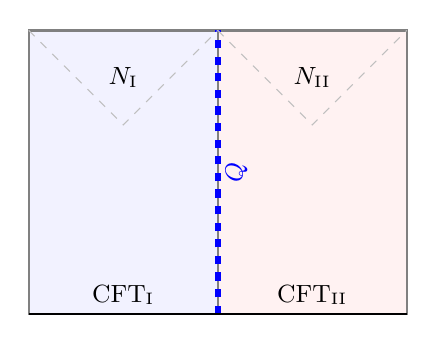
\begin{tikzpicture}[scale=1.2]
    % Left bulk (N_I)
    \draw[fill=blue!5, draw=gray, thick] (0,0) rectangle (2,3);
    \node at (1,2.5) {\small $N_{\text{I}}$};
    
    % Right bulk (N_II)
    \draw[fill=red!5, draw=gray, thick] (2,0) rectangle (4,3);
    \node at (3,2.5) {\small $N_{\text{II}}$};
    
    % Interface brane Q (blue vertical line)
    \draw[thick, blue, line width=2pt, dashed] (2,0) -- (2,3);
    \node[blue, rotate=90] at (2.2,1.5) {\small $Q$};
    
    % CFT labels at the boundary
    \node at (1,0.2) {\small CFT$_{\text{I}}$};
    \node at (3,0.2) {\small CFT$_{\text{II}}$};
    
    % Optional: Add boundary line at the bottom
    \draw[black, thick] (0,0) -- (4,0);
    
    % Optional: Add perspective lines
    \draw[gray!50, dashed] (0,3) -- (1,2) -- (2,3);
    \draw[gray!50, dashed] (2,3) -- (3,2) -- (4,3);
\end{tikzpicture}
\end{document}